\section{Controlled numerical illustrations}\label{sec:experiments}
The numerical study uses oracle Gaussian velocities and explicit nonlinear conditional kernels. Its purpose is to expose the distinctions proved above and check quantitative formulas in reproducible settings. Every Gaussian $W_2$ value is obtained from its covariance formula. For nonlinear fields we report a theorem-based bound and a Monte Carlo estimate of the cost of a specified coupling, not an estimate of an optimal transport distance. The explicit calculations are generated by \texttt{experiments/reproduce.py}; the trained experiment below is generated independently by \texttt{experiments/learn\_operator.py}.

\subsection{A positive autonomy defect and its endpoint consequence}
For \Cref{ex:gaussian}, we evaluate the integrated defect by adaptive quadrature with absolute and relative tolerances $2\times10^{-12}$. We integrate the matrix ODE $\dot F_s=A_sF_s$, $F_0=I$, using DOP853 with relative tolerance $10^{-11}$ and absolute tolerance $10^{-13}$. The restricted field replaces the first row by $((2s-1)/a_s,0)$ and keeps the second row unchanged. It is the exact population minimizer under the coarse-autonomy restriction.

The terminal covariance is $FF^T$. For positive semidefinite matrices $A,B$, the centered Gaussian distance is \citep{gelbrich1990}
\begin{equation}\label{eq:gaussian-w2}
 W_2^2(\mathcal N(0,A),\mathcal N(0,B))
 =\tr\left(A+B-2(B^{1/2}AB^{1/2})^{1/2}\right).
\end{equation}
The unrestricted covariance agrees with the target to less than $7\times10^{-13}$ in maximum entrywise error for all four correlations considered. The conditional refinement map \eqref{eq:conditional-gaussian-map} has the target covariance algebraically.

\begin{table}[htbp]
\centering\small
\begin{tabular}{rrrrr}
\toprule
$\rho$ & $D_P(1/2)$ & $\int_0^1D_P(s)\,ds$ & Endpoint $W_2$ & Correlation \\
\midrule
0.25 & 0.031746 & 0.012520 & 0.088539 & 0.127354 \\
0.50 & 0.133333 & 0.053524 & 0.177729 & 0.270978 \\
0.80 & 0.380952 & 0.165833 & 0.281233 & 0.516544 \\
0.95 & 0.582728 & 0.298427 & 0.303295 & 0.757538 \\
\bottomrule
\end{tabular}

\caption{Gaussian bridge obstruction. The final two columns refer to the restricted global velocity, not to conditional refinement. Conditional refinement has zero endpoint error analytically. The integrated defect is a squared-velocity quantity and is not an endpoint-distance lower bound.}\label{tab:gaussian}
\end{table}
\begin{figure}[tb]
\centering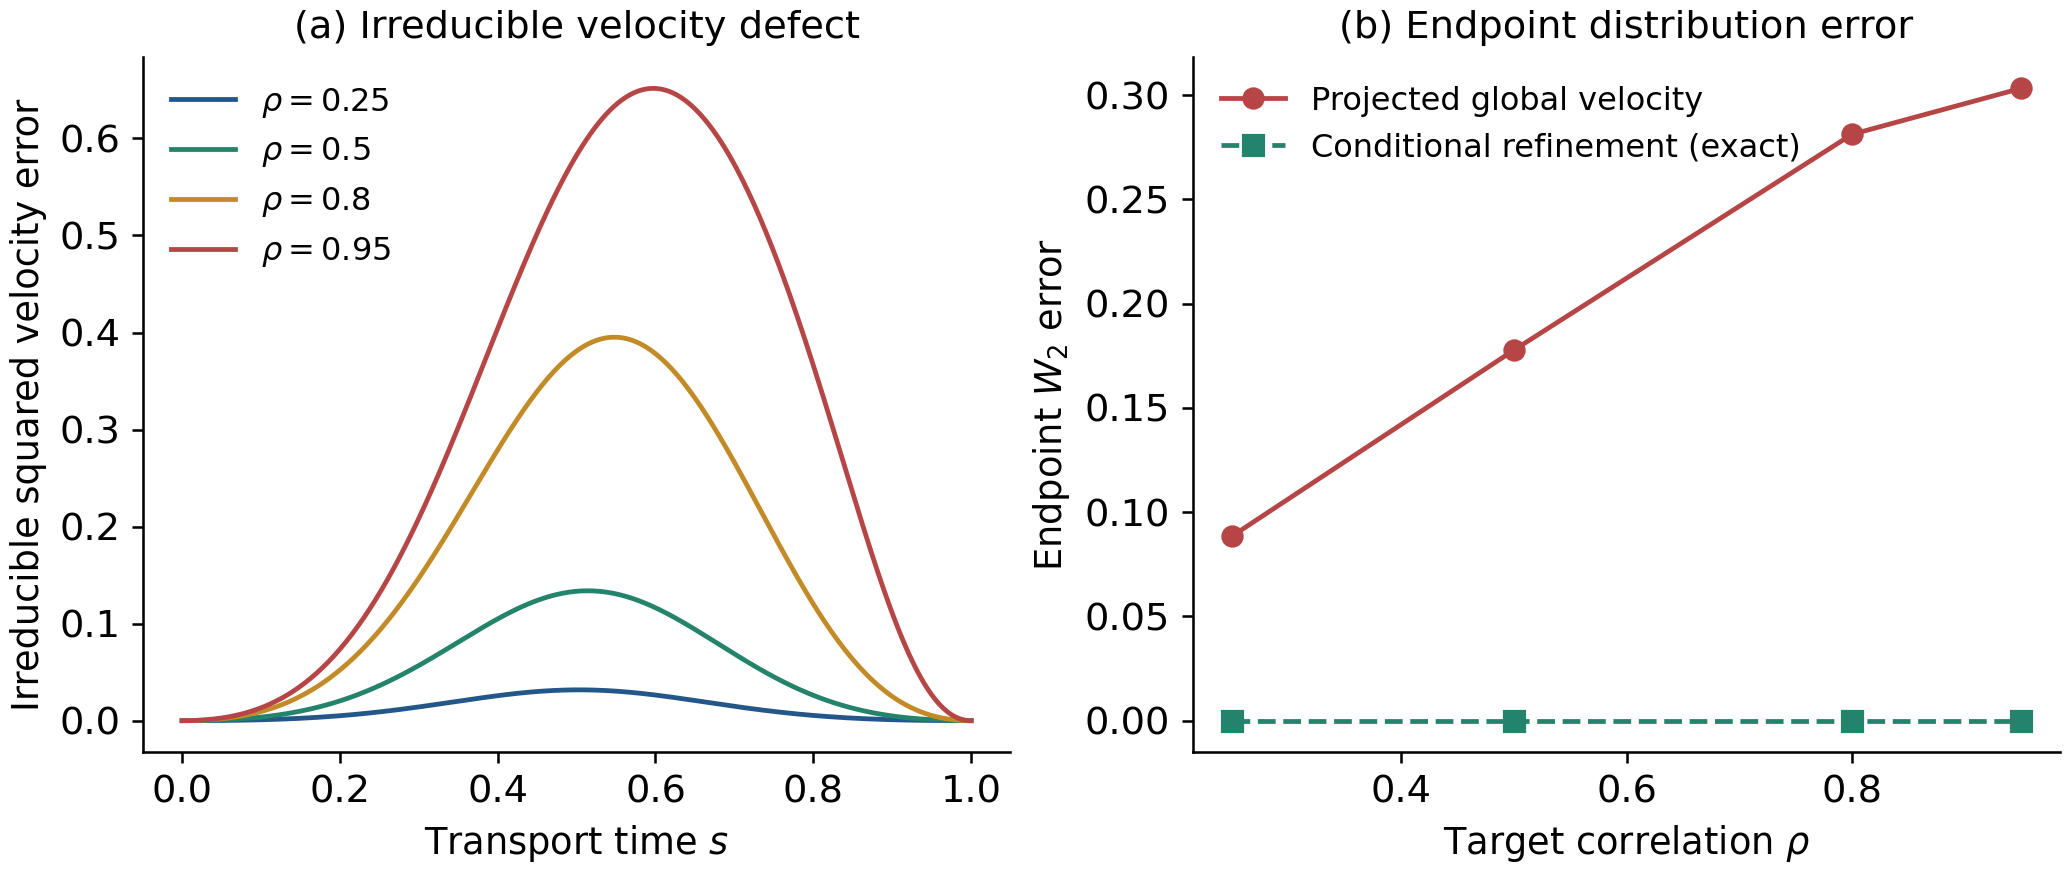
\includegraphics[width=\textwidth]{figures/bridge_obstruction.png}
\caption{Left: the exact irreducible defect $D_P(s)$ of the specified global bridge. Right: endpoint distances after integrating its unrestricted fine row and optimal coarse-only row, compared with the exact conditional refinement endpoint.}\label{fig:defect}
\end{figure}

For $\rho=0.8$, the restricted endpoint covariance is approximately
\begin{equation}
 \widehat\Sigma=
 \begin{pmatrix}
 1.000000&0.467279\\
 0.467279&0.818350
 \end{pmatrix}.
\end{equation}
It has correlation $0.516544$ and $W_2$ error $0.281233$. The observed coordinate has the correct marginal variance, but the cross-coordinate law has changed. This example makes the difference between matching projected marginals and matching a joint law directly visible.

\begin{figure}[tb]
\centering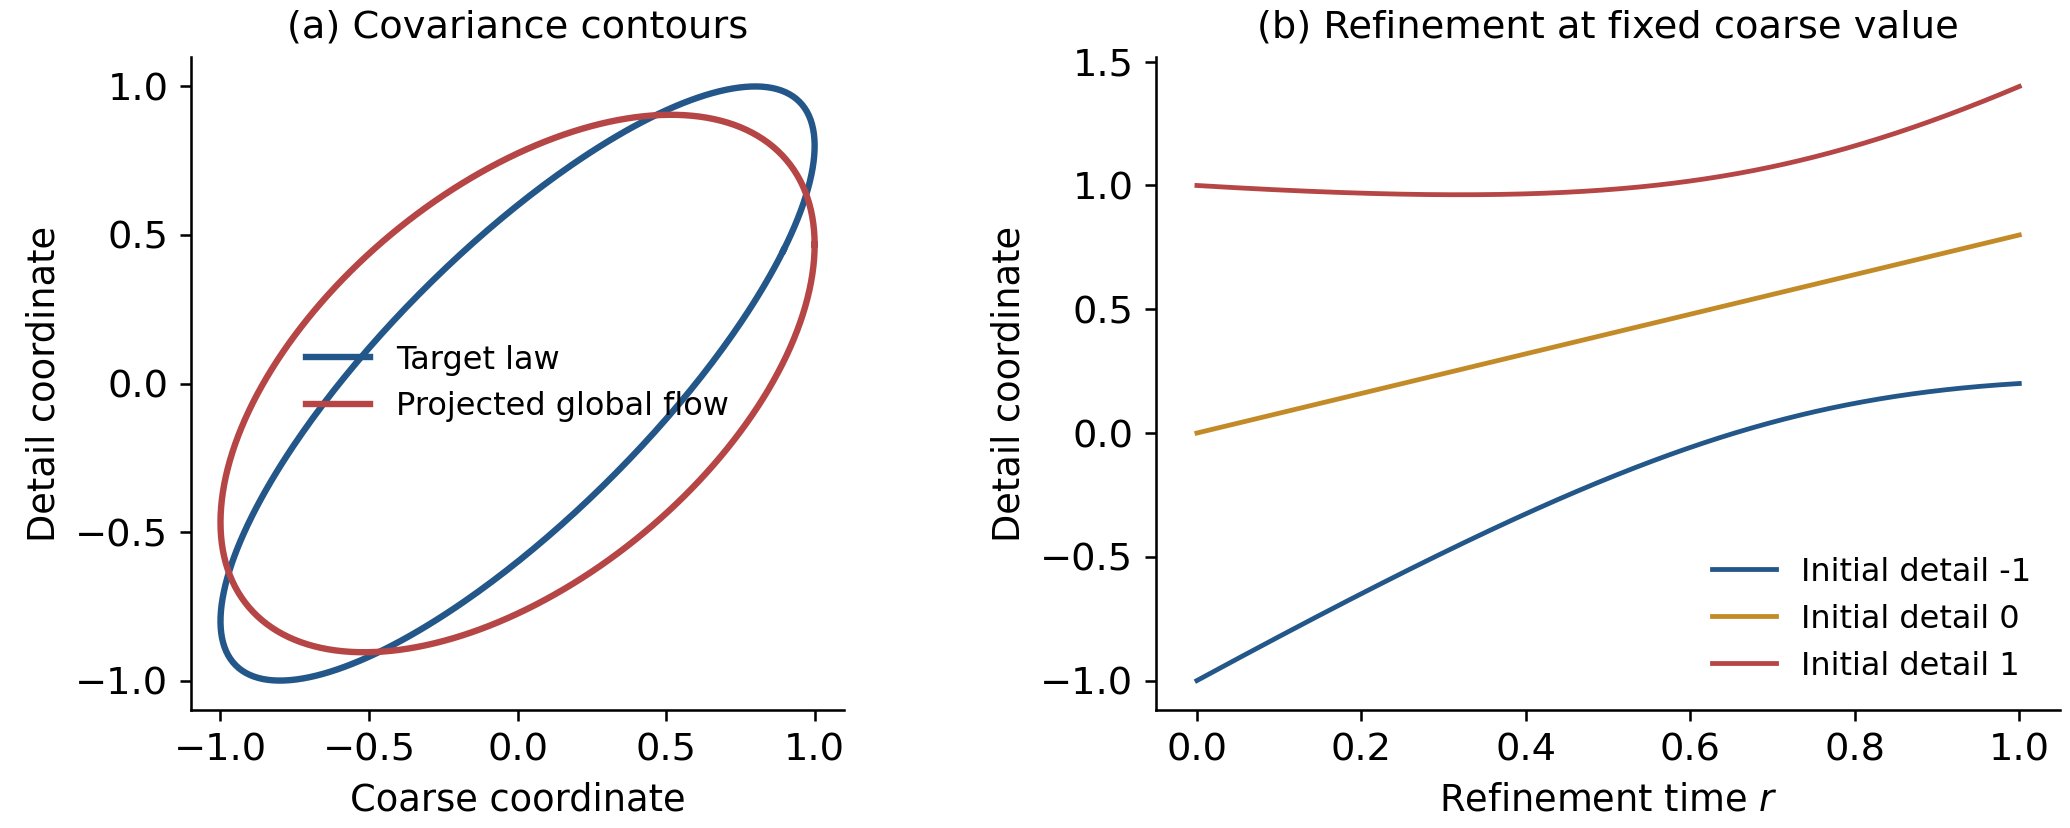
\includegraphics[width=.96\textwidth]{figures/conditional_refinement.png}
\caption{For $\rho=0.8$, the restricted global flow changes the covariance contour (left). Conditional refinement holds the sampled coarse value fixed and transports only the detail coordinate; the displayed paths use coarse value $x=1$ and three initial detail values (right).}\label{fig:conditional}
\end{figure}

\subsection{A nonlinear coherent field with an explicit accuracy certificate}
Let $H=L^2(0,1)$ with orthonormal sine basis $e_j(x)=\sqrt2\sin(j\pi x)$. Here modes are indexed by $j=1,2,\ldots$, a shift of the abstract band's initial index $0$. Define
\begin{align}\label{eq:synthetic-field}
 U_1&=\xi_1,\\
 U_j&=\frac{0.6\tanh(U_1)+0.4\tanh(U_{j-1})+\xi_j}{j},
 \qquad j\ge2,\qquad \xi_j\overset{\mathrm{iid}}\sim\mathcal N(0,1),\notag\\
 U&=\sum_{j\ge1}U_je_j.\notag
\end{align}
The conditional mean in the numerator has absolute value at most one. Since $\xi_j$ is independent of its context, $\E U_j^2\le2/j^2$ for $j\ge2$. Thus $U\in L^2(\Omega;H)$ and
\begin{equation}\label{eq:synthetic-tail}
 \tau_m^2\le2\sum_{j>m}j^{-2},\qquad m\ge1.
\end{equation}
To create an approximate conditional generator with known error, retain the first mode exactly and use
\begin{equation}\label{eq:perturbed-field}
 \widehat U_j=
 \frac{0.6\tanh(\widehat U_1)+0.4\tanh(\widehat U_{j-1})+\beta+(1+\delta)\xi_j}{j},
 \qquad \beta=0.08,\quad\delta=0.12.
\end{equation}
At the same context, the true and approximate conditional laws are Gaussian and
\begin{equation}\label{eq:synthetic-constants}
 \eps_j=\frac{\sqrt{\beta^2+\delta^2}}{j},\qquad
 L_2=\frac12,\qquad L_j\le\frac{\sqrt{0.52}}{j}\quad(j\ge3).
\end{equation}
For $j=2$, both context terms act on the same first coordinate; for later modes their gradients occupy distinct coordinates, explaining the two Lipschitz formulas. Both required square sums are finite. The theorem therefore applies to the infinite field, not just to its numerical truncation.

We use $60{,}000$ independent innovation sequences with seed $20260911$, retain a 256-mode target reference, and share each sequence between the true and approximate recursions. The coupling RMS in \Cref{tab:refinement} estimates
\begin{equation}\label{eq:coupling-mc}
 \left(\E\norm{P_{256}U-\widehat U^{(m)}}^2\right)^{1/2},
 \qquad \widehat U^{(m)}=\sum_{j=1}^m\widehat U_je_j.
\end{equation}
Its population value is an upper bound on the finite-reference $W_2$ distance. The empirical value is a sampling estimate of that bound. The last column is the deterministic full-law certificate $\sqrt{2\sum_{j>m}j^{-2}+d_m^2}$, which includes the infinite target tail.

\begin{table}[htbp]
\centering\small
\begin{tabular}{rrrr}
\toprule
Modes & Coupling RMS$^{\dagger}$ & $d_m$ & Full-law bound \\
\midrule
2 & 0.688046 & 0.072111 & 0.891666 \\
4 & 0.511363 & 0.111139 & 0.674535 \\
8 & 0.377030 & 0.133628 & 0.502872 \\
16 & 0.278531 & 0.145792 & 0.377400 \\
32 & 0.209868 & 0.152123 & 0.290989 \\
64 & 0.163959 & 0.155352 & 0.234822 \\
128 & 0.134965 & 0.156982 & 0.200518 \\
256 & 0.117721 & 0.157802 & 0.180828 \\
\bottomrule
\end{tabular}

\caption{Nonlinear refinement. $^{\dagger}$Monte Carlo estimate of the specified coupling RMS to a 256-mode target reference; it is not an optimal Wasserstein distance. $d_m$ is the exact recursively computed certificate. The last column bounds $W_2$ to the infinite target law.}\label{tab:refinement}
\end{table}
At $m=256$, the estimated coupling RMS is $0.117721$, the refinement certificate is $0.157802$, and the full-law bound is $0.180828$. The Monte Carlo standard error of the \emph{squared} coupling cost is $3.42\times10^{-5}$ at this resolution. Full values and standard errors are included in \texttt{results/metrics.json}. The separation between conditional error and tail error in \Cref{fig:certificate} reflects \eqref{eq:pythagorean-certificate}.

\begin{figure}[tb]
\centering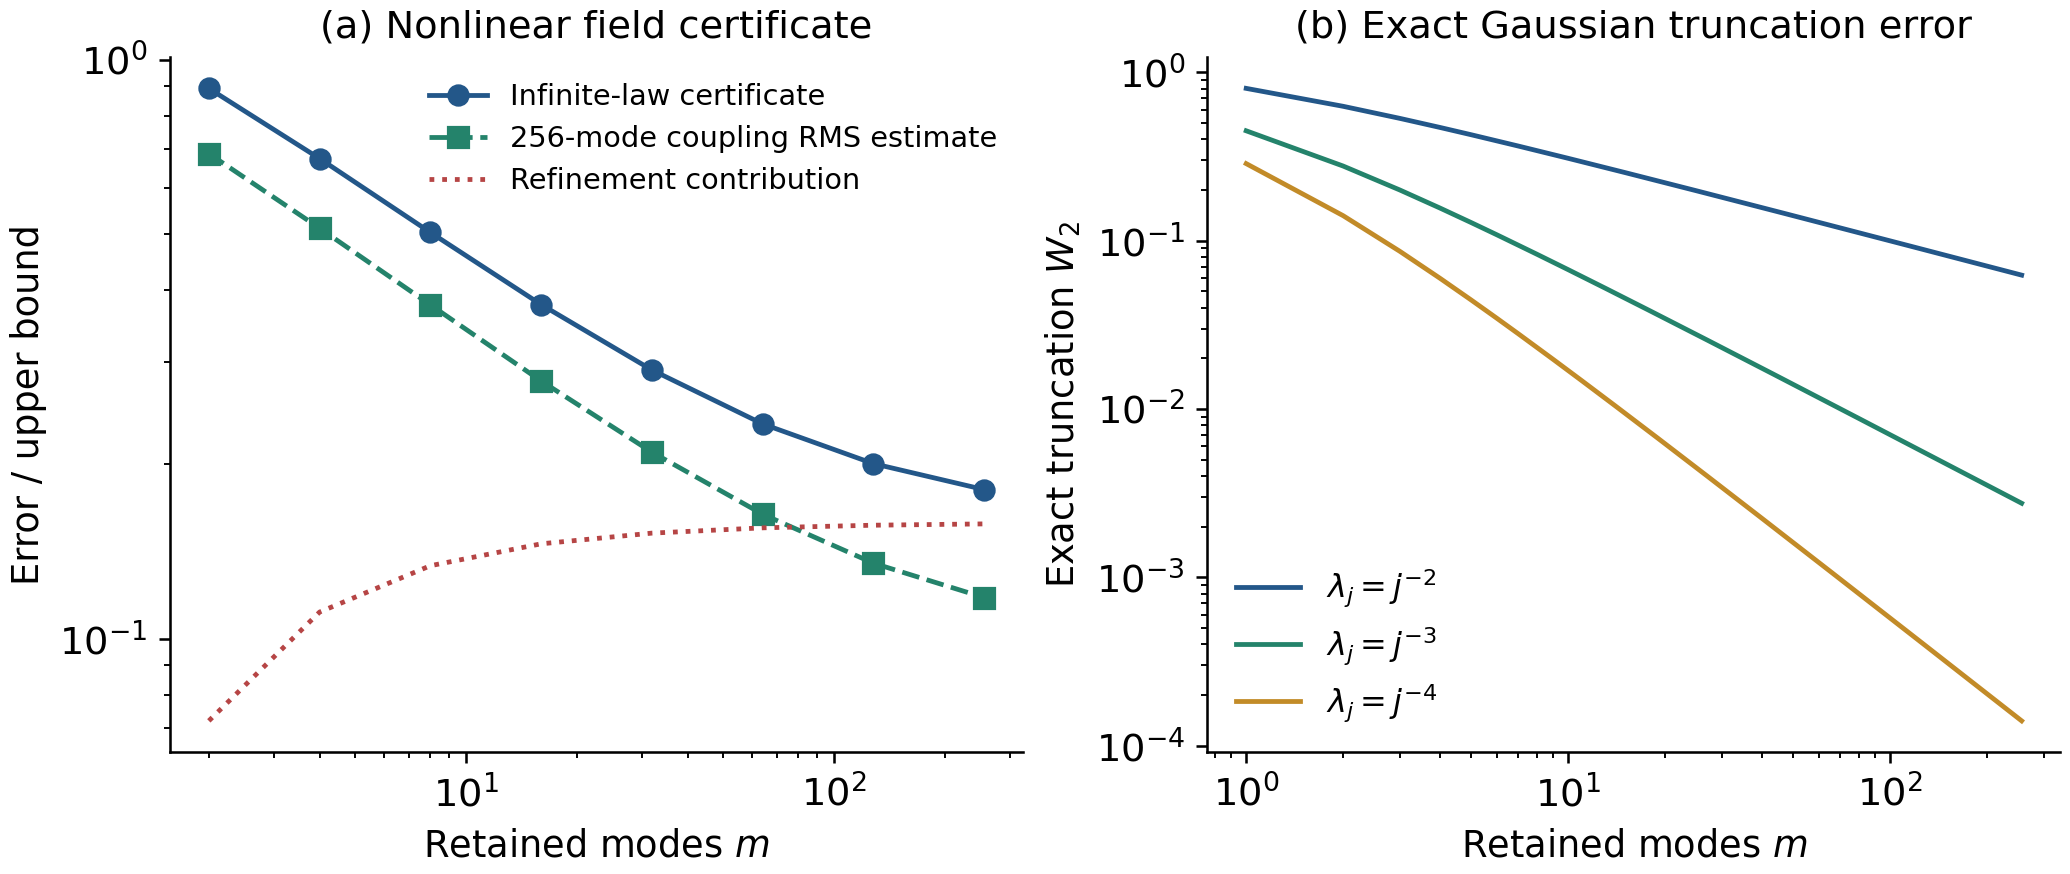
\includegraphics[width=\textwidth]{figures/refinement_certificate.png}
\caption{Left: full-law error certificates, refinement contributions, and estimated finite-reference coupling costs for the nonlinear field. Right: exact Gaussian truncation distances for three covariance spectra. These tail distances apply to generation in the retained linear subspace.}\label{fig:certificate}
\end{figure}
\begin{figure}[tb]
\centering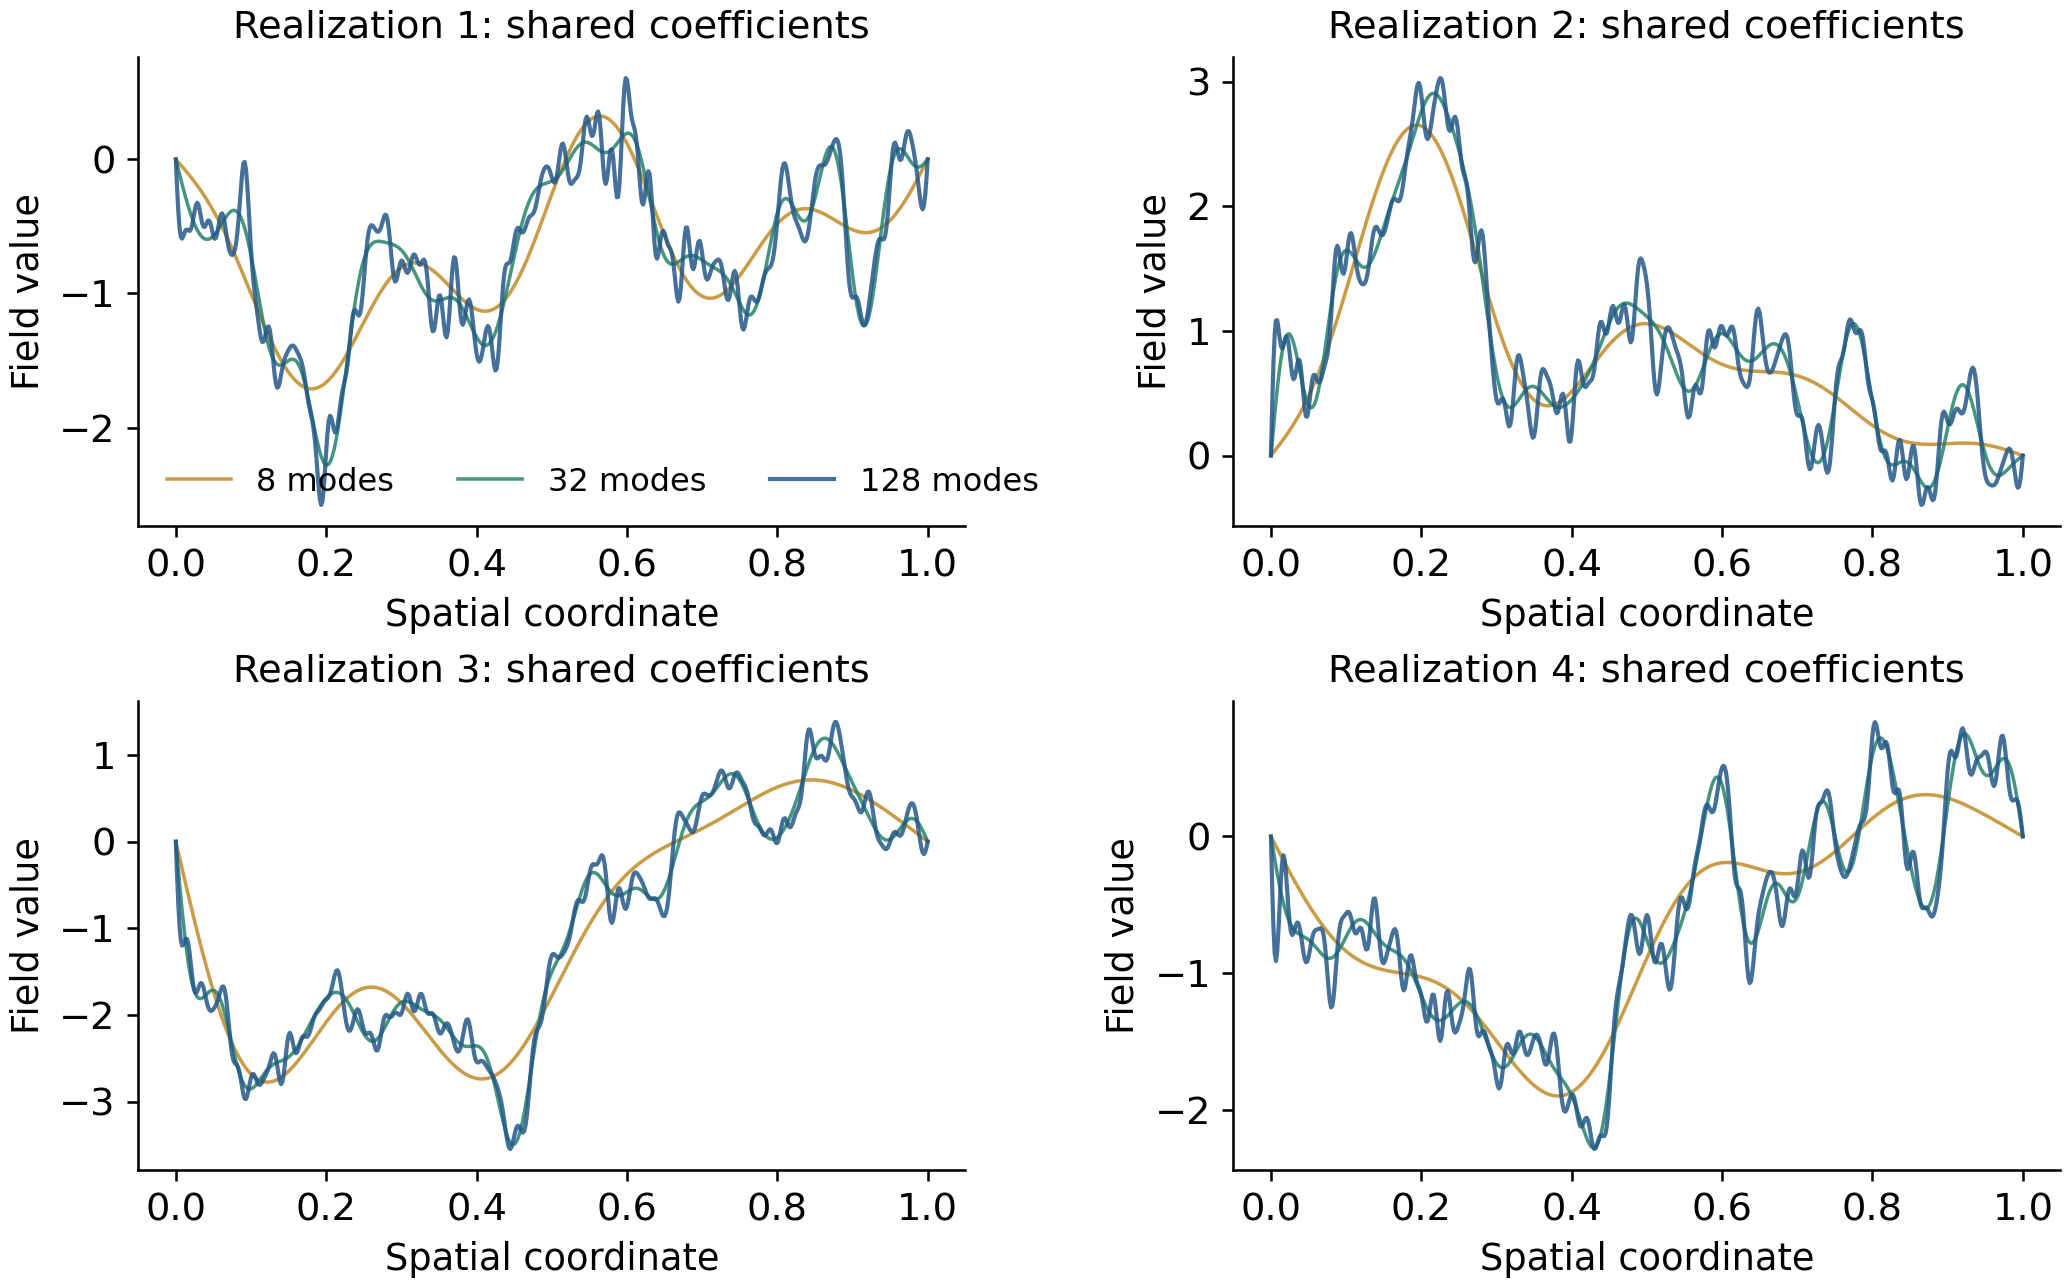
\includegraphics[width=\textwidth]{figures/coherent_fields.png}
\caption{Four realizations of the nonlinear target at 8, 32, and 128 modes using shared innovations. Lower coefficients are exactly unchanged by refinement. The curves are finite sine-series reconstructions; convergence claims in the paper concern the $L^2$ state norm.}\label{fig:fields}
\end{figure}

\subsection{A trained shared generator and simultaneous validation}\label{sec:learned-experiment}
We now learn the conditional generator for \eqref{eq:synthetic-field}. The model is \eqref{eq:neural-detail} with twelve hidden units, a softmax vector of positive output weights, and a learned positive innovation scale. It has 37 trainable parameters shared across every mode. The first mode is sampled exactly. Each hidden row is projected onto the Euclidean ball of radius $1.3$ after every update; the innovation scale is constrained to $[0.7,1.3]$.

For each of three preselected seeds, training uses 8,192 independent noisy target fields observed through mode 32. There are 1,800 Adam steps of 2,048 context/detail pairs, with learning rate $0.012$. Half the sampled pairs use mode 2 and the rest sample modes 3--32 uniformly. The objective is Gaussian conditional negative log-likelihood for the normalized coefficient $jU_j$. Conditional means are not supplied as training labels. There is no validation-based hyperparameter or seed selection.

An independent audit contains 65,536 fields through mode 256. Because the synthetic conditional mean is known, it evaluates the bounded loss in \Cref{sec:validation} with $B_j=4$. The $K=3$ candidate networks and all 255 detail modes share an overall failure probability $\delta=0.01$. The global sensitivity uses the actual learned value $K_\theta=\sum_kp_k\|a_k\|$, not a Jacobian measured at a few validation points. The values for the three runs are $0.966423$, $0.965939$, and $1.024007$; their innovation scales are $0.994923$, $1.005759$, and $0.985614$.

\begin{table}[htbp]
\centering\small
\begin{tabular}{rrrrr}
\toprule
Modes & Coupling RMS & Estimated $d_m$ & 99\% $d_m$ & 99\% full-law bound \\
\midrule
8 & 0.36176 & 0.01201 & 0.04367 & 0.48676 \\
16 & 0.25508 & 0.01283 & 0.04824 & 0.35143 \\
32 & 0.17553 & 0.01323 & 0.05065 & 0.25318 \\
64 & 0.11550 & 0.01343 & 0.05189 & 0.18357 \\
128 & 0.06724 & 0.01352 & 0.05251 & 0.13536 \\
256 & 0.00908 & 0.01357 & 0.05283 & 0.10290 \\
\bottomrule
\end{tabular}

\caption{The first preselected training seed. Coupling RMS is an empirical cost to the 256-mode target reference, and estimated $d_m$ plugs empirical conditional errors into the recurrence. The last two columns use simultaneous 99-percent conditional-error bounds; only the final column also includes the infinite target tail.}\label{tab:learned}
\end{table}

At mode 256, the empirical projected coupling RMS is respectively $0.009081$, $0.006697$, and $0.025350$. The full-law confidence bounds are $0.102899$, $0.102447$, and $0.109925$. The distinction is material: the conservative unresolved target-tail bound alone is $0.088302$, and statistical confidence also enlarges the conditional-error inputs. The standard errors of the squared coupling costs are recorded in the numerical file; they do not replace the population confidence calculation.

A separately retrained ablation removes the previous-band input while retaining the first coordinate. Its 256-mode coupling RMS is $0.105823$. Removing all mean context, while preserving the target innovation scale, gives $0.417298$. These controlled ablations isolate the value of conditional information within the stated field model. They do not rank this architecture against diffusion models or neural operators trained on other datasets.

\begin{figure}[tb]
\centering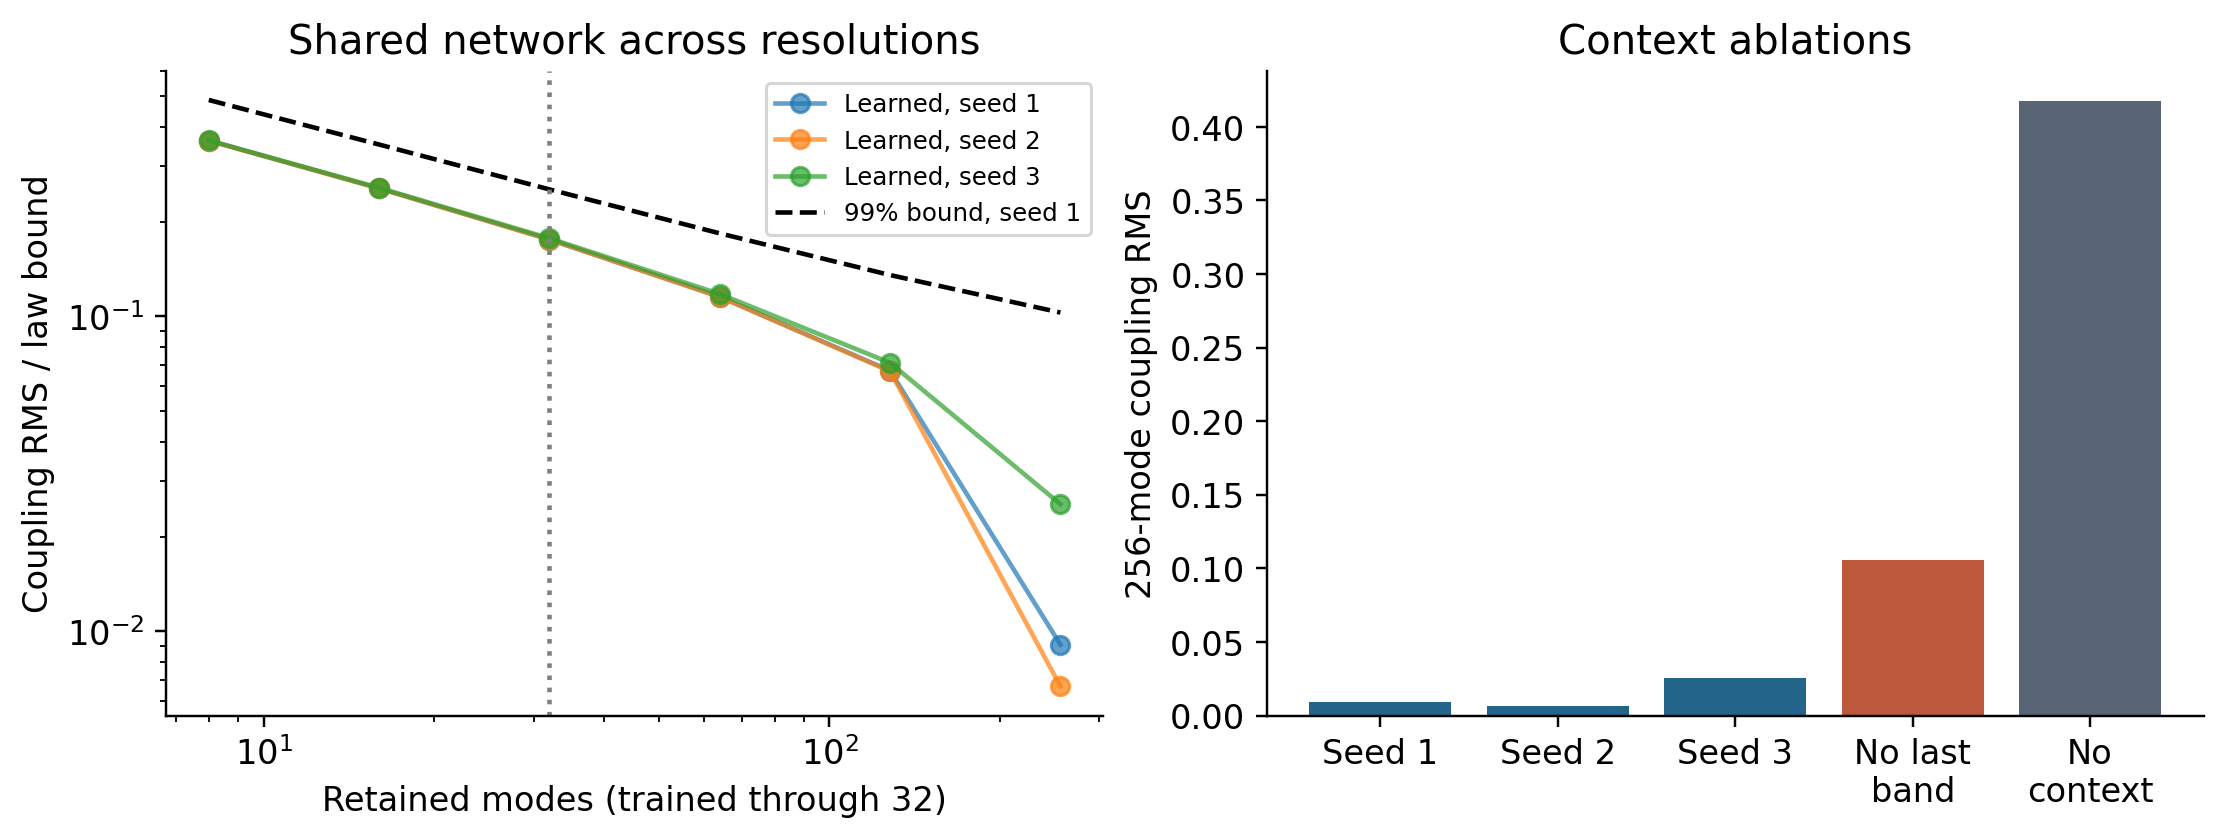
\includegraphics[width=\textwidth]{figures/learned_operator.png}
\caption{A neural model trained through 32 modes and audited through 256. The left panel distinguishes empirical finite-reference coupling costs from the first seed's full-law confidence bound. The right panel compares all three seeds with context ablations. Shared innovations reproduce every retained coefficient exactly when additional modes are requested.}\label{fig:learned}
\end{figure}

The supplied CPU float64 program records every training seed, objective, constraint, fitted parameter, bandwise fitting estimate, confidence input, and context bound. The audit uses new target fields beyond the training cutoff, so this experiment tests resolution extrapolation with known conditional laws. It does not claim that unobserved fine-scale laws can be inferred from coarse data without the structural assumptions stated in the model.

\subsection{An audit that uses observed fields without conditional-mean labels}
To test \Cref{thm:observed-audit,thm:dependency}, use the sine basis above with
\begin{equation}\label{eq:bounded-observed-field}
 U_1=X,\qquad U_j=\frac{m(X)+0.1\xi_j}{j}\quad(j\ge2),\qquad
 m(x)=0.7\tanh(0.8x)+0.1\sin(3x),
\end{equation}
where $X,\xi_2,\ldots$ are independent uniform variables on $[-1,1]$.
The first coefficient is a sufficient context for every later band. The target mean obeys $|m|\le0.8$ and $\Lip(m)\le0.86$. The target tail satisfies
$\tau_m^2\le(0.8^2+0.1^2/3)\sum_{j>m}j^{-2}$.

Three networks, with seeds $481,482,483$, each have twelve slopes and twelve softmax weights:
$f_\theta(x)=\sum_{k=1}^{12}p_k\tanh(a_kx)$.
The slopes are constrained to $[-1.3,1.3]$, giving the exact implemented sensitivity $\sum_kp_k|a_k|$. Each network trains on $16{,}384$ noisy fields through eight modes, using $1{,}200$ Adam steps and batches of $1{,}024$ randomly chosen field-mode pairs. The regression target is the observed normalized coefficient $jU_j$, not $m(X)$. Generation uses $(f_\theta(X)+0.1\xi_j)/j$. A fourth, predeclared candidate has $f=0$. All candidates share the known noise scale; learning an unspecified noise law would require a different model fit, although the distributional audit itself can compare more general scalar laws.

Two independent audit splits use seeds $7401,7402$. For budgets $n=4{,}096$, $16{,}384$, and $65{,}536$ fields per split, the feature partitions have respectively eight, twelve, and sixteen equal cells. These choices are fixed before the audit; the total failure budget $0.01$ is divided across the three budgets. Within each budget, the union bounds cover all four candidates and all 31 audited detail bands, hence every retained cutoff. Dependence between modes of one field is allowed. No cell is empty in the realized datasets; the code nevertheless implements the diameter bound for empty cells.

Both target and learned normalized details lie in $[-1.1,1.1]$. The empirical-to-model transport has a closed formula. For sorted observations $z_{(i)}$, $i=1,\ldots,n$, and a uniform model on $[c-\sigma,c+\sigma]$,
\begin{equation}\label{eq:empirical-uniform}
 W_2^2\!\left(\frac1n\sum_i\delta_{z_i},\operatorname{Unif}[c-\sigma,c+\sigma]\right)
 =\frac1n\sum_i\left[z_{(i)}-c-\sigma\left(\frac{2i-1}{n}-1\right)\right]^2
 +\frac{\sigma^2}{3n^2}.
\end{equation}
This follows by integrating the squared difference of the two quantile functions on each interval of length $1/n$. Thus the audit evaluates observed detail distributions against the learned kernel directly. It receives the support and regularity assumptions but never calls the target-mean function. Floating-point evaluation of the formula is kept distinct from a formally rounded numerical enclosure.

Because the sole parent coordinate is sampled exactly, \Cref{thm:dependency} combines the certified fitting inputs in quadrature. For seed 481 at $m=32$ and the largest budget, the generic prefix recurrence gives $0.908405$, whereas the dependency certificate gives $0.585551$. This improvement uses a proved architectural restriction, not a smaller confidence budget. Across all three trained seeds the latter bound ranges from $0.585268$ to $0.587704$. The no-context bound is $0.723932$.

\begin{table}[htbp]
\centering\small
\begin{tabular}{rrrrr}
\toprule
Fields per split & Cells & Learned bound & No-context bound & Coupling upper \\
\midrule
4,096 & 8 & 1.0304 & 1.0632 & 0.0633 \\
16,384 & 12 & 0.7653 & 0.8687 & 0.0633 \\
65,536 & 16 & 0.5856 & 0.7239 & 0.0633 \\
\bottomrule
\end{tabular}

\caption{Observed-data certification at 32 modes. The learned columns use the predeclared seed 481. Every bound includes a justified infinite target tail and belongs to the simultaneous 99\% event. The final column is a separate numerical evaluation of a specified full-law coupling, using the synthetic truth only for this diagnostic; it is not the audit input or an optimal transport distance.}\label{tab:observed-audit}
\end{table}
\begin{figure}[htbp]
\centering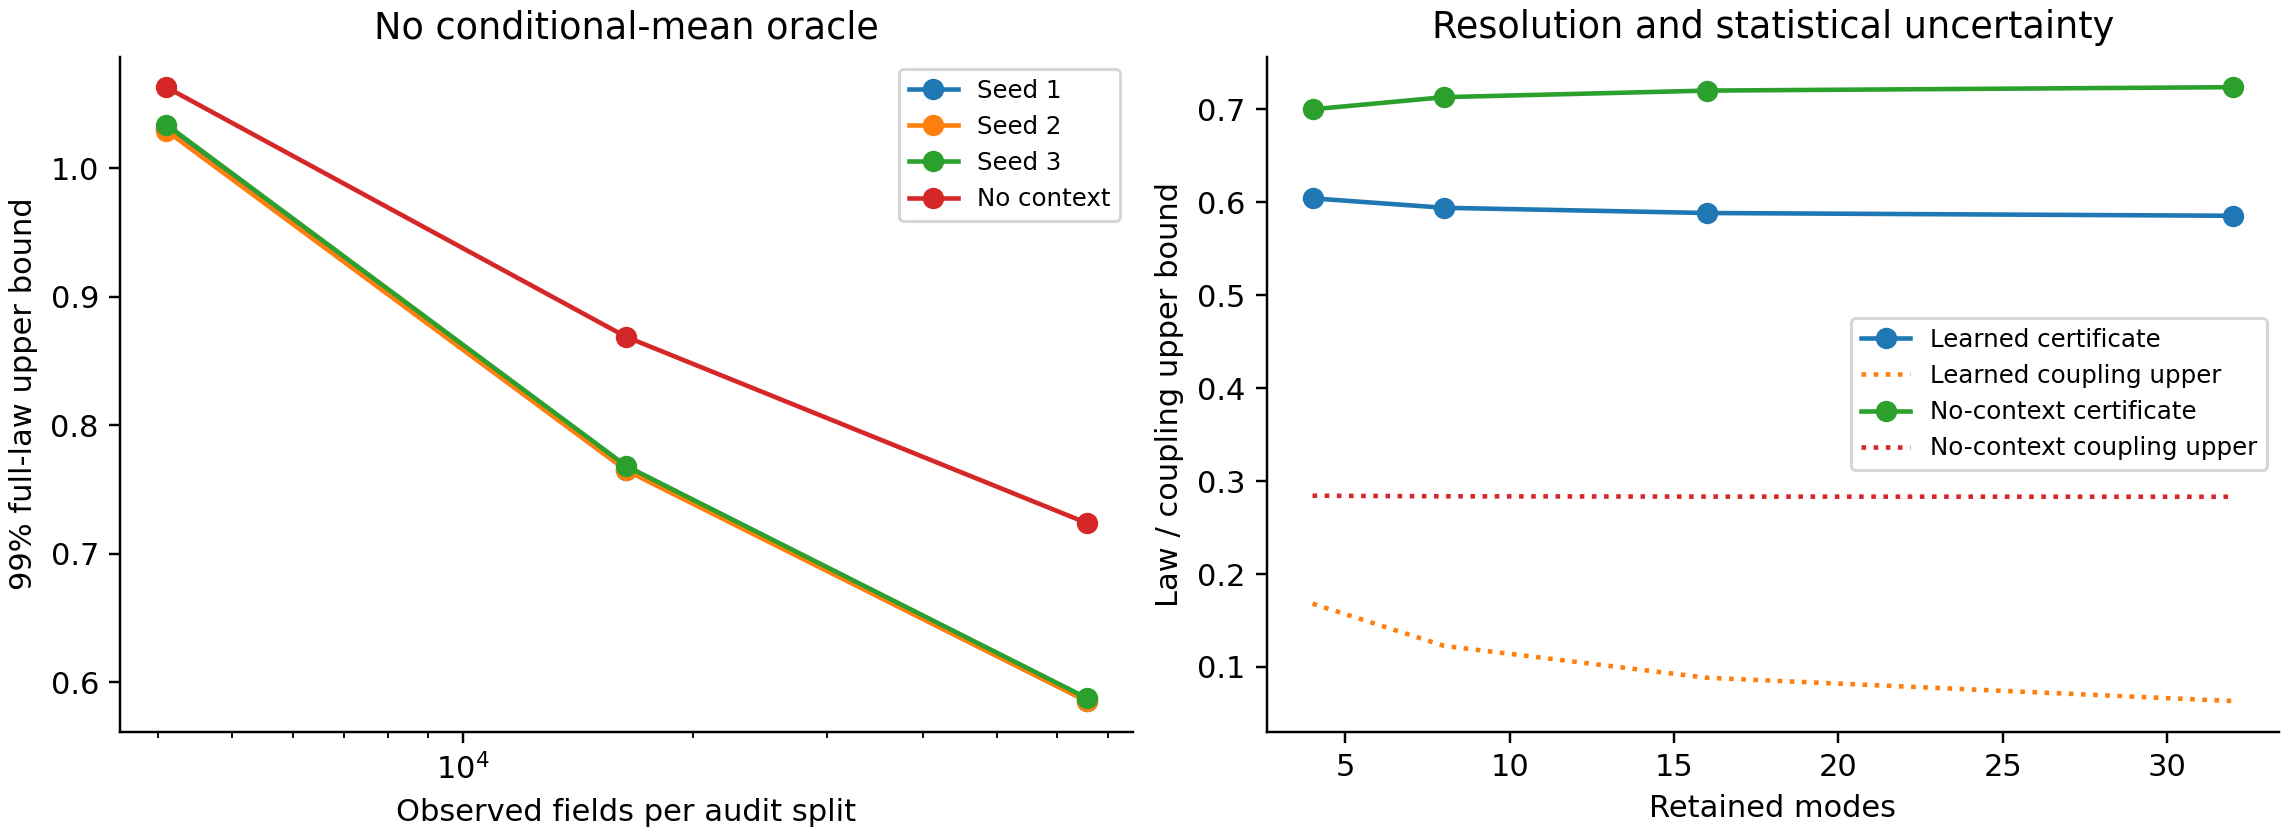
\includegraphics[width=\textwidth]{figures/observed_audit.png}
\caption{Observed-data audit with two independent splits. Left: all three trained seeds and the no-context candidate. Right: the dependence on retained resolution at the largest budget. Dotted lines evaluate a specified coupling using the known synthetic law; solid lines include statistical uncertainty and the deterministic tail envelope.}\label{fig:observed-audit}
\end{figure}

The actual conditional mean discrepancy is evaluated only in a separate truth diagnostic. Sharing $X$ and every uniform innovation makes each retained detail discrepancy $(m(X)-f_\theta(X))/j$. A 512-point Gauss--Legendre integral computes its squared mean; repeating with 1,024 points changes it by less than $10^{-15}$. For seed 481, the resulting full-law coupling upper estimate at 32 modes is $0.0633$. The much larger statistical certificate exposes the price of distribution-free cellwise estimation, the support envelope, and simultaneous coverage. The bound is informative as a guaranteed radius under the assumptions, but is not a precise estimator of the attained error. The target's analytic tail envelope also exceeds its actual tail. The code records both the generic and dependency recursions, every bandwise confidence input, cell occupancy, and all trained parameters.

\subsection{A geometry check for overlapping coordinates}
\Cref{fig:observation-geometry} evaluates the exact two-coordinate example in \Cref{sec:riesz}. The aligned discrepancy $x=y$ has squared physical-to-coordinate error ratio $1+c$, while the encoder's condition number is $\sqrt{(1+c)/(1-c)}$. The two quantities answer different questions: the former transfers a forward approximation bound, and the latter measures the worst relative instability of recovering coordinates. The plot checks the analytic formulas; it is not a fitted neural experiment.
\begin{figure}[htbp]
\centering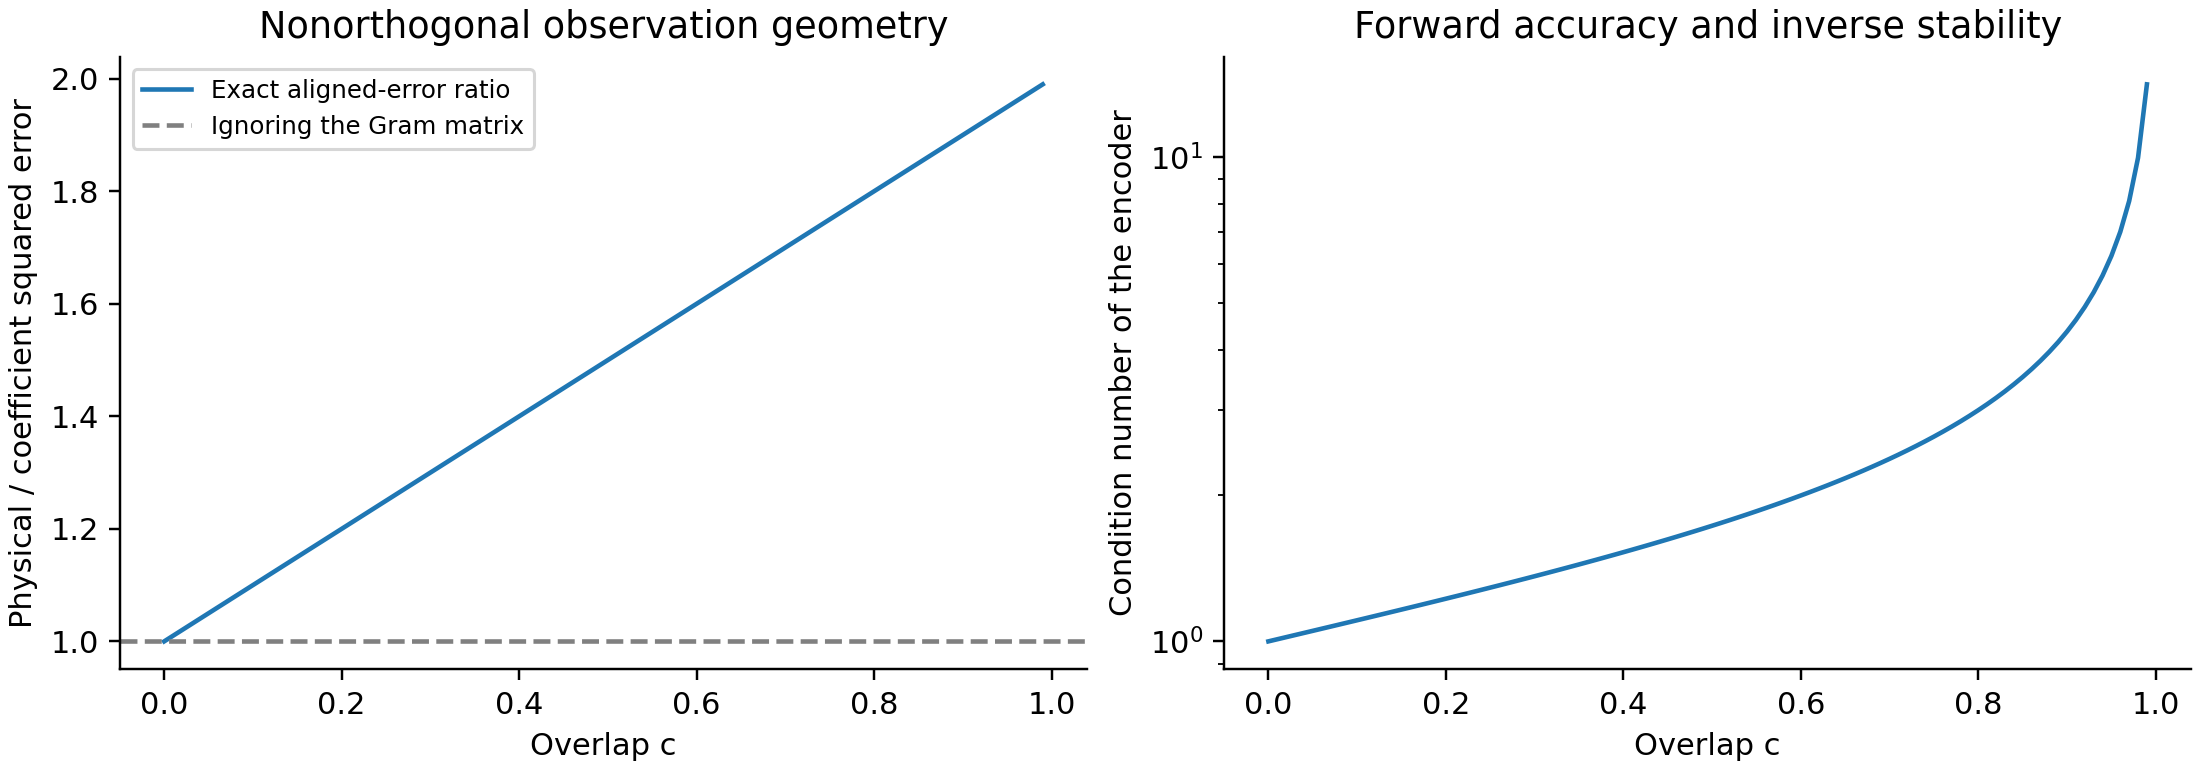
\includegraphics[width=\textwidth]{figures/observation_geometry.png}
\caption{Overlapping observation coordinates. Forward error distortion can remain bounded while the inverse representation becomes arbitrarily ill-conditioned.}\label{fig:observation-geometry}
\end{figure}


\subsection{Reproducibility and scope of numerical verification}
The script checks the orthogonal transport identity for correlated Gaussian coordinates, the sharp deterministic construction in \Cref{prop:sharpness}, the Gaussian off-diagonal defect formula, and the conditional Gaussian ODE endpoint. Their observed absolute residuals are, respectively, approximately $7.1\times10^{-15}$, zero at floating-point precision, below $2\times10^{-13}$ over the tested parameter grid, and $1.4\times10^{-12}$. These checks support implementation and arithmetic; the mathematical proofs establish the general statements.

The explicit examples isolate the bridge obstruction and sharpness mechanisms. The Gaussian trained experiment adds noisy-data fitting and a conditional-mean-based validation certificate. The bounded-field experiment uses observed conditional distributions, with no target-mean call inside its audit. Its support, sufficient context, regularity constants, and tail envelope are explicit assumptions. Both studies report all predeclared seeds. The numerical programs test implementations; the proofs establish the stated universal results.
